% Jacobian-as-linear-map schematic for notebook 03.
% Unit ball of joint rates -> manipulability ellipsoid in task (twist) space.
% Standalone: compiles with `lualatex jacobian_map.tex`; loaded via render_tikz_file.
\documentclass[tikz,border=4pt]{standalone}
\usepackage{amsmath}
\usepackage{amssymb}
\usepackage{tikz}
\usetikzlibrary{arrows.meta,calc}
\begin{document}
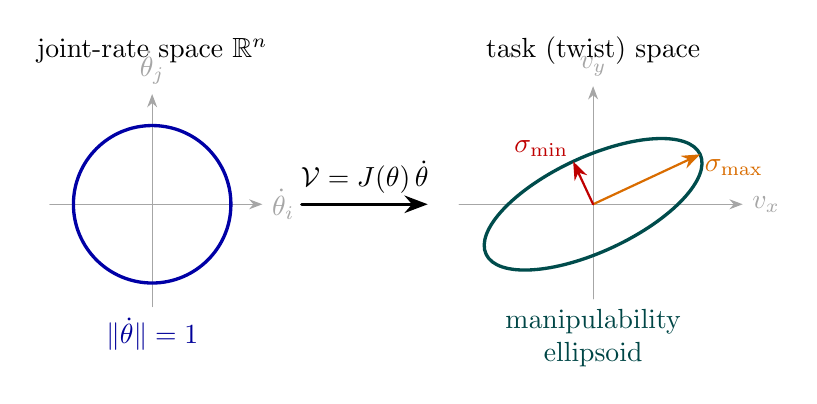
\begin{tikzpicture}[>=Stealth, line cap=round, line join=round, scale=1.0]

  % --- left: unit ball of joint velocities ---
  \begin{scope}[shift={(0,0)}]
    \draw[->,gray!70] (-1.3,0) -- (1.4,0) node[right]{$\dot\theta_i$};
    \draw[->,gray!70] (0,-1.3) -- (0,1.4) node[above]{$\dot\theta_j$};
    \draw[blue!65!black, very thick] (0,0) circle (1.0);
    \node[blue!60!black] at (0,-1.65) {$\|\dot\theta\|=1$};
    \node at (0,1.95) {joint-rate space $\mathbb{R}^n$};
  \end{scope}

  % --- map arrow ---
  \draw[->, line width=1.2pt] (1.9,0) -- (3.5,0)
        node[midway,above]{$\mathcal{V}=J(\theta)\,\dot\theta$};

  % --- right: manipulability ellipsoid (image of the ball) ---
  \begin{scope}[shift={(5.6,0)}]
    \draw[->,gray!70] (-1.7,0) -- (1.9,0) node[right]{$v_x$};
    \draw[->,gray!70] (0,-1.2) -- (0,1.5) node[above]{$v_y$};
    \draw[teal!60!black, very thick, rotate=25] (0,0) ellipse (1.5 and 0.6);
    % principal axes = singular values
    \draw[->,orange!85!black,thick,rotate=25] (0,0) -- (1.5,0)
          node[below right=-2pt]{$\sigma_{\max}$};
    \draw[->,red!75!black,thick,rotate=25] (0,0) -- (0,0.6)
          node[above left=-2pt]{$\sigma_{\min}$};
    \node at (0,1.95) {task (twist) space};
    \node[teal!55!black, align=center] at (0,-1.7)
         {manipulability\\ ellipsoid};
  \end{scope}
\end{tikzpicture}
\end{document}
